Acuity Scheduling~\cite{acuity} describes itself as \enquote{an online appointment-booking tool} that \enquote{is great for any business that needs clients to book appointments for services in advance.} It also says that \enquote{businesses including yoga studios, massage therapists, acupuncture, life coaches, photographers, hair and nail salons use Acuity with great success,} but that it \enquote{is not a great fit for businesses that want to book appointments that last more than a day, like car rentals, vacation rentals, or hotels.} Acuity Scheduling is a subsidiary of Squarespace -- a company that primarily focuses on providing a website-building service (for some time after Squarespace acquired Acuity, the scheduling product was rebranded to Squarespace Scheduling, but that change has since been reverted).

The website offers a free limited-time trial, after which it cannot be used without paying for one of its tiered plans. After first singing up for a business account, the user is asked for the name of their business and the name of an Acuity Scheduling subdomain that the service will create for the booking website of the business (this is optional, and if not provided, the website will be available under a shared subdomain and a URL query parameter with a generated identifier).

The user then creates their first appointment type by filling out the name of the appointment, its duration, whether it is a one-on-one appointment or a group appointment, and optionally, its price. If the user has selected the group appointment type, they must set the number of open slots per class as well.

Moreover, the user sets up the availability of the created appointment type by selecting a date and a time, whether or not it is a recurring event, and, if it is, the frequency of the recurrence (such as every Monday, every other Tuesday, the first Wednesday of each month, or daily), and the number of recurrences.

Lastly, the user can optionally connect third-party payment processors (Stripe, Square, and PayPal) for collecting deposits or full payments for the appointment bookings. Long-term subscriptions are also supported. The service claims~\cite{acuity} that it does not take any commission on the payments and that the only fees are those charged by the payment processor.

After the business user completes the sign-up process, customers can access a booking website that is created for the business. Upon accessing the website, customers see the business information (with only the sign-up completed, that is just the business name), followed by a list of appointments to choose from, with each appointment featuring its name, time and date, duration, and a sign-up button. If the business user selected the group appointment type, there is also a quantity field above the appointment list and the number of free spots available under each appointment's sign-up button. Signing up for a selected appointment is followed by filling out personal information (a full name, an email address, and optionally a phone number). If there was no payment required, the customer completes the booking and receives an email with the details of their booking, a link to reschedule or cancel the appointment, and links to add the appointment to their calendar. The booking page can be seen in the figure~\ref{fig:acuity_scheduling}. The customer can use an account to manage their booked appointments, but it is purely optional, and they can still manage their bookings through the email links. There is also no way for the business to limit their appointments to only signed-in customers (the business can, however, ban clients by their email address).

The scheduling functionality can be integrated into any website built with Squarespace (which can then use a custom domain). There are also simple booking components that can be embedded into another website, in addition to the option to embed a booking page iframe. The booking website can be customized by choosing between a couple of predefined layouts and can also use custom CSS. The platform also features webhooks and an extensive application programming interface (API), which can be used to integrate it with other applications.

Business users can see all their appointments in a calendar overview, as well as all their clients. Under each appointment in the calendar, the user can see all signed-up customers, reschedule or cancel their bookings (when the business user does this, the affected customer can be notified by email, but there is also an option not to send this notification), and add private notes and tags for each customer. The user can manually add new attendees to each appointment (which can be useful, for example, when a customer wants to create a booking over the phone, but the business wants to have everything tracked in the booking system). There is also an option to send an email to all attendees of a selected appointment, in addition to SMS reminders. The business user can be notified of new activity by email as well, and they can synchronize their calendar with other popular calendar applications.

Appointment types can be further customized by adding a color and a picture. Users can make appointments private, in which case they are not visible to the public and can only be accessed through a direct link. There is an option to require clients to sign up for every recurrence of a recurring appointment and an option to disallow clients from booking multiple spots. Appointment types can also have a form added for the customers to fill out before booking an appointment. The form can consist of questions with answers of several different types, including a text field, a drop-down list, a checkbox, and even a file upload. The business information shown on the booking website can also be customized a bit further by, for instance, adding a logo, filling out rich content instructions for the customers, and changing to one of a few different languages.

Other features available include CSV import and export of clients and appointments, setting limits on how long before an appointment it can be canceled or rescheduled, and adding Google Analytics to the booking website. A business account may be used by multiple users with separate login credentials and role-based permissions.

\begin{figure}
    \centering
    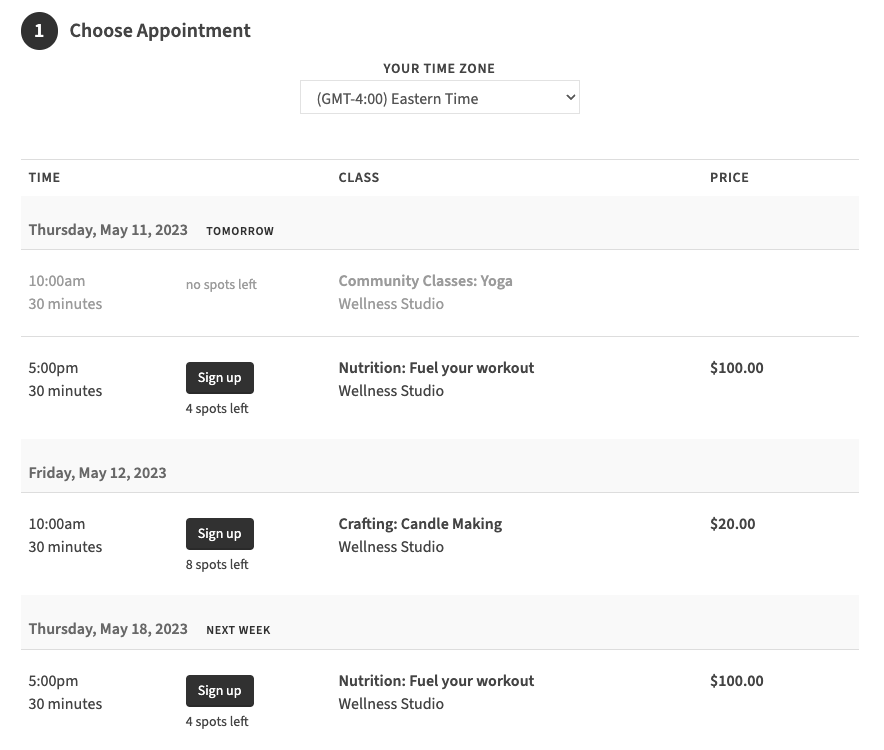
\includegraphics[width=1.0\textwidth]{content/existing_reservation_systems/acuity_scheduling.png}
    \caption[Acuity Scheduling]{Acuity Scheduling~\cite{acuity}}
    \label{fig:acuity_scheduling}
\end{figure}
